

\chapter{Results}

In this chapter, we describe the results from our pose and depth experiments. In Chapter 3 we described an unsupervised pipeline for learning depth and visual odometry from monocular imagery. Similarly, in Chapter 4 we adapted conventional 2D machine learning techniques to apply 4D image data to learning these tasks. Specifically, we recommended two variants of an algorithm for learning depth and visual odometry from light fields - the first uses all the information from the light field to generate a novel rendering of a single \textit{U, V} slice, while the second method uses the known configuration of the camera array to create a rendering of the complete light field. In this chapter, we contrast results for three algorithms - each of the two novel pipelines described in Chapter 4, and the existing monocular approach described in Chapter 3. For the two algorithms that we have suggested, we also evaluate three ingestion methods: focal-stacks, volumetric images, and tiled EPI images. 

First, we evaluate each algorithm's performance in pose-estimation, and demonstrate results for cumulated trajectories for several input-sequences. Subsequently, we'll evaluate the algorithms' performance in depth-prediction and photometric reconstruction. 


\section{Experimental Setup Details}
In each of our experiments, we use the same training dataset of 9000 grayscale input images consisting of 48 short video-sequences. The testing set, which is also the same across all experiments, consists of ~400 input images over 4 video-sequences. For training we use a batch size of 2 images, and train for a total of 300 epochs. 


\section{Pose Estimation and Visual Odometry}

An important metric of error is the \textit{absolute instantaneous error} for each of the 6 degrees-of-freedom that are estimated. This metric describes the magnitude of the error between the predicted and the true component. As described in Chapter 4, we have collected ground-truth pose data using a robotic manipulator platform with a repeatability of $\pm 0.01$ millimeters. Meanwhile, we can evaluate each pipeline's effectiveness in estimating the \textit{average cumulative error} by comparing the true trajectory with the predicted trajectory. 

\subsection{Single-View Reconstruction Approach}



\begin{figure}[H]
    \centering
    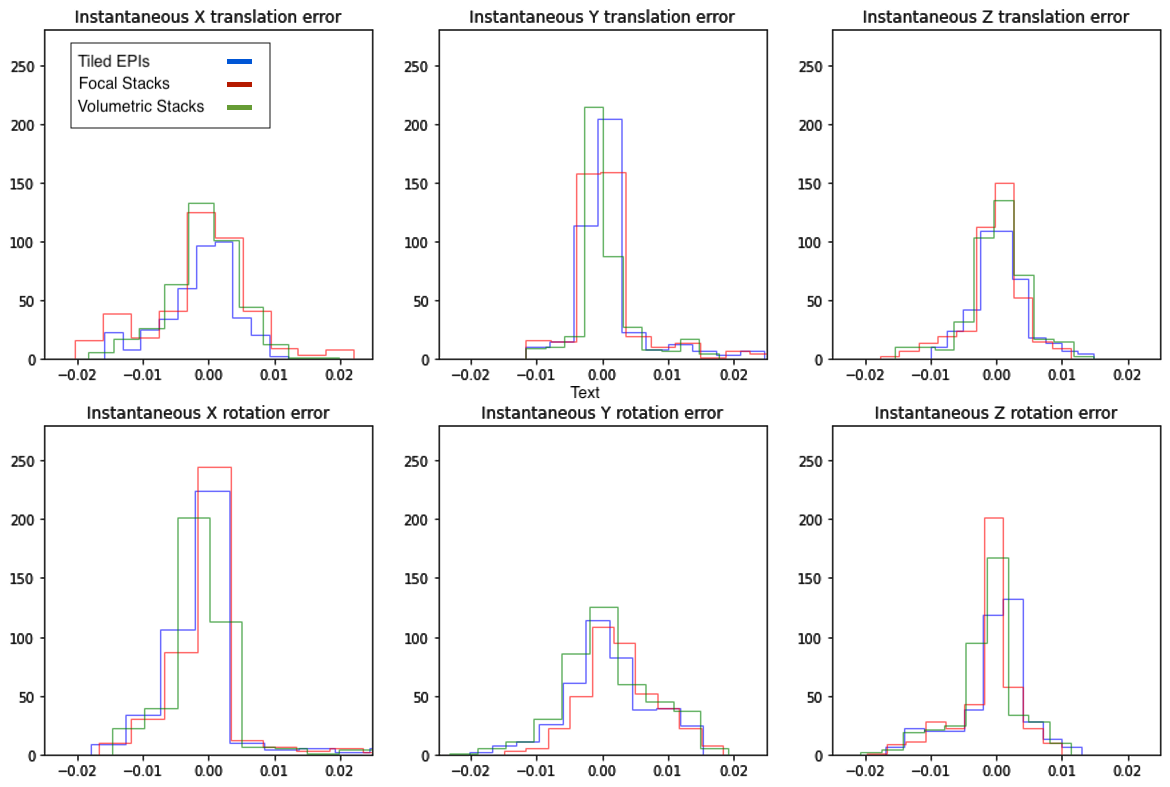
\includegraphics[width=\textwidth]{images/result-examples/pose/errors/sw_comparison_hist.png}
    \caption[Histograms of instantaneous errors for each input method, using single-view reconstruction]{Histograms of instantaneous absolute errors, comparing our three input methods. Importantly, while the error histograms exhibit reasonably tight distributions, some outliers exist. Outliers such as these are likely to impact the cumulative error over the complete trajectory, due to the cumulative nature of odometry errors. Comparing these histograms, a decisive winner is not immediately apparent. Table 5.1 summarises the mean errors, from which we might conclude that the tiled EPI format has performed best.}
\end{figure}

The histogram in Figure 5.1 summarises 400 observations of the absolute instantaneous error for each of the 6 degrees of freedom (translation and rotation in X, Y and Z), over three input methods (tiled epipolar images, focal stacks, and volumetric stacks). 

Figures 5.2 and 5.3 show two examples of true and estimated trajectories for the three input methods, as well as the existing monocular method. 

\begin{figure}[H]
    \centering
    \hspace*{-3cm}
    \subfloat[Tiled EPIs]{
        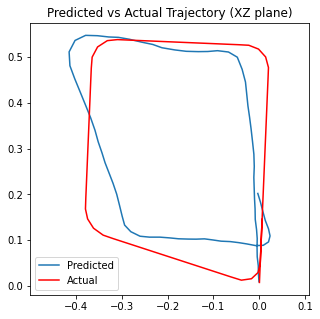
\includegraphics[height=1.8in]{images/result-examples/pose/trajectories/singlewarp/sw-epi-16.png}
    }
    \subfloat[Focal Stacks]{
        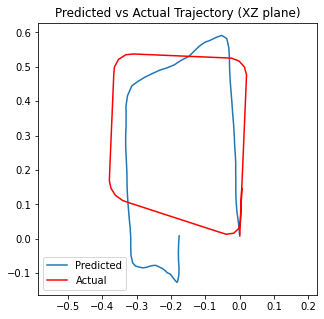
\includegraphics[height=1.8in]{images/result-examples/pose/trajectories/singlewarp/sw-focalstack-175-16.png}
    }
    \subfloat[Volumetric Images]{
        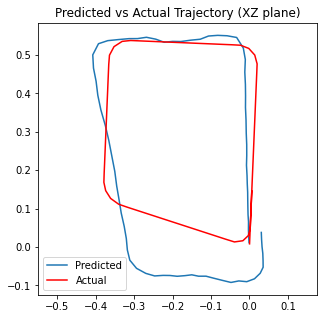
\includegraphics[height=1.8in]{images/result-examples/pose/trajectories/singlewarp/sw-stack-16.png}
    }
    \subfloat[Monocular]{
        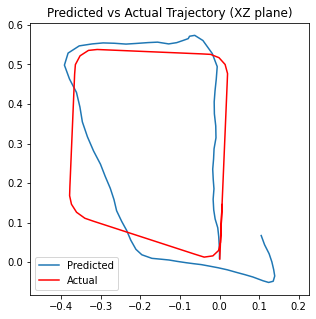
\includegraphics[height=1.8in]{images/result-examples/pose/trajectories/monocular/monocular-16.png}
    }\\
    \caption[Estimated and true trajectories for input sequence 16 using single-view reconstruction]{Estimated and true trajectories for input sequence 16. Inspecting these traces, there is no clear consensus over which input format best reconstructs the path. Qualitatively, we suggest that (b) - Focal Stacks, exhibits the poorest fit for the true path.}
    \setcounter{subfigure}{0}

    \centering
    \hspace*{-3cm}
    \subfloat[Tiled EPIs]{
        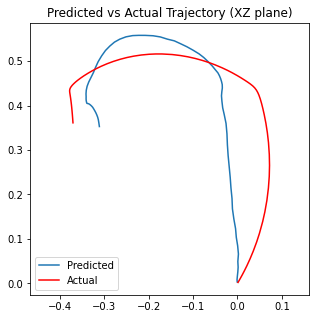
\includegraphics[height=1.8in]{images/result-examples/pose/trajectories/singlewarp/sw-epi-44.png}
    }
    \subfloat[Focal Stacks]{
        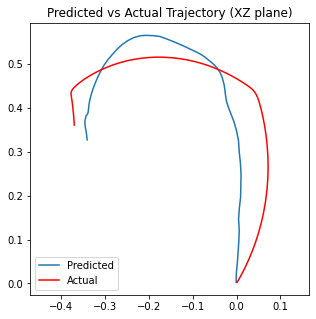
\includegraphics[height=1.8in]{images/result-examples/pose/trajectories/singlewarp/sw-focalstack-175-44.png}
    }
    \subfloat[Volumetric Images]{
        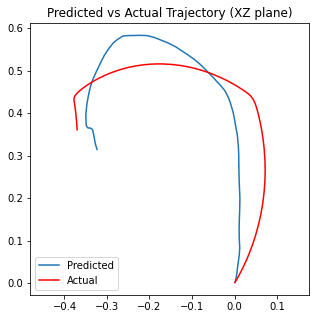
\includegraphics[height=1.8in]{images/result-examples/pose/trajectories/singlewarp/sw-stack-44.png}
    }
    \subfloat[Monocular]{
        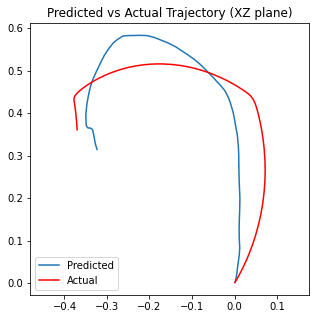
\includegraphics[height=1.8in]{images/result-examples/pose/trajectories/monocular/monocular-44.png}
    }
    \caption[Estimated and true trajectories for input sequence 44 using single-view reconstruction]{Estimated and true trajectories for input sequence 44. Qualitatively, these results are competitive with existing approaches. Once again, there is no qualitative consensus over which input format reconstructs the paths best. Inspecting Table 5.1 however we see that quantitatively, on average, tiled EPIs exhibit the smallest error.}
    \setcounter{subfigure}{0}
\end{figure}

Importantly, in Figure 5.2 (d) and 5.3 (d), we have shown trajectories estimated by the existing monocular approach. Our results using light field imagery are qualitatively competitive with existing monocular approaches, and we demonstrate quantitatively in Section 5.2.3 that our approach using light fields in fact outperforms the monocular approach. 


Table 5.1 summarises the instantaneous and cumulative errors for the three input methods. 
 
\begin{table}[htbp]
    \caption{Mean Absolute Instantaneous Error and Cumulative Error}
    \centering
    \begin{tabular}{@{}lcc@{}}
        \toprule
        Input Method        & Absolute Instantaneous Error (mm)   & Cumulative Error (mm) \\
        \midrule 
        Tiled EPIs & \textbf{9.64} & \textbf{71.38} \\
        Focal Stacks & 9.79 & 104.03 \\
        Volumetric Stacks & 12.17 & 103.47 \\
        Monocular & 12.90 & 122.23 \\
        \bottomrule
        
    \end{tabular}
\end{table}

The fact that using light field imagery produces improved trajectory results compared to monocular imagery is unsurprising. Multiple view imaging offers rich geometric information about the scene, and our three suggested input methods are all arranged in a way such that simple 2D features relating to parallax and depth may be easily learned by a 2D convolutional filter. Monocular imagery on the other hand forces a convolutional network to learn semantic features relating to depth - we might expect a network trained on monocular imagery to learn roughly what the size of a stuffed animal is, and use the size of the image it forms on the sensor plane to estimate its distance from the camera. These extra steps are not necessary when using multiple view imaging because the depth of the stuffed animal is encoded directly as 2D features that can be learnt, circumventing any of the guesswork that a monocular approach requires. We elaborate more on the difference between monocular and light field imagery in Chapter 6. In the next section, we once again investigate how these input methods perform, after modifying the reconstruction pipeline to reconstruct the complete light field, rather than a single viewpoint from the center of the camera module. 

\newpage


\subsection{Light Field Reconstruction Approach}

\begin{figure}[h]
    \centering
    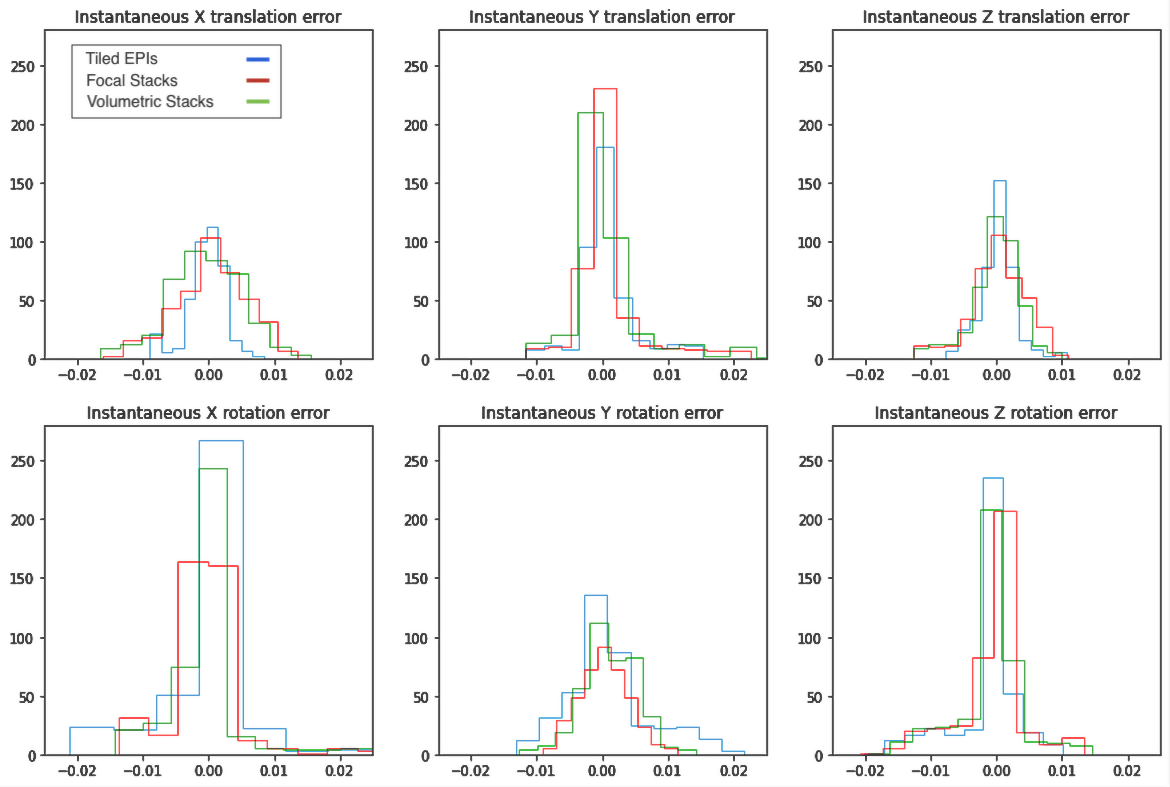
\includegraphics[width=\textwidth]{images/result-examples/pose/errors/mw_comparison_hist.png}
    \caption[Histogram of instantaneous errors for each input method, using light field reconstruction]{Histograms of instantaneous absolute errors comparing our three input methods. In general, we observe that the error distributions using the light field reconstruction approach are generally tighter with shorter tails, compared with the single-view reconstruction approach. We also observe that the distributions of our three input methods indicate that the tiled EPI format performs best - consistently exhbiting the highest peaks around 0.}
\end{figure}

Here we describe the performance of the second variant of our suggested pipeline, using the known camera configuration to photometrically warp the complete light field. Because this pipeline incorporates known information about the relationship between individual sub-apertures on the camera module, we expect this pipeline to demonstrate improved performance in pose estimation and scale-awareness.

We carry this expectation because this variant of the pipeline generates a stronger supervision signal - the larger number of pixels being warped results in a significantly heavier loss for the same error, compared with the single-view reconstruction approach. Additionally, this variant carries a much smaller tolerance to scale inconsistencies due to the constraints imposed when incorporating multiple sub-apertures and their known relative spacing.

Once again, we attach our analysis to a comparison to the monocular approach. Figures 5.5 and 5.6 both show a comparison to the trajectories generated by the monocular approach, as well as our three input methods.


\begin{figure}[H]
    \centering 
    \hspace*{-1.5cm}
    \subfloat[Tiled EPIs]{
        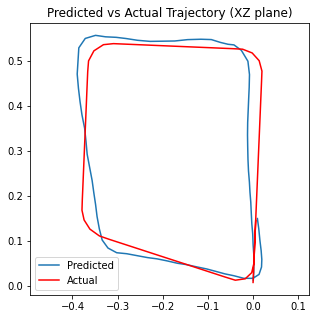
\includegraphics[height=1.8in]{images/result-examples/pose/trajectories/multiwarp/mw-epi-16.png}
    }
    \subfloat[Focal Stacks]{
        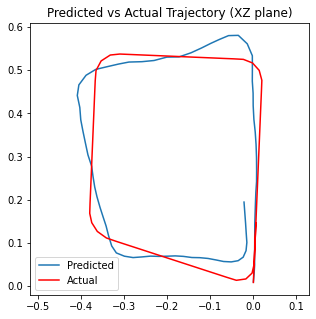
\includegraphics[height=1.8in]{images/result-examples/pose/trajectories/multiwarp/mw-fs-175-16.png}
    }
    \subfloat[Volumetric Images]{
        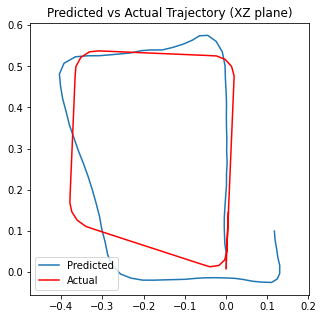
\includegraphics[height=1.8in]{images/result-examples/pose/trajectories/multiwarp/mw-stack-16.png}
    }
    \subfloat[Monocular]{
        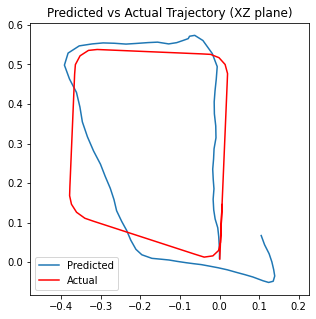
\includegraphics[height=1.8in]{images/result-examples/pose/trajectories/monocular/monocular-16.png}
    }
    \caption[Estimated and true trajectories for input sequence 16 using light field reconstruction]{Estimated and true trajectories for input sequence 16. Here, we see that tiled EPIs qualitatively outperform the other methods. In general, each of the three input methods using light field imagery are competitive with the existing monocular approach, with Table 5.2 indicating that these methods all outperform monocular imagery.}
    \setcounter{subfigure}{0}
    \centering 
    \hspace*{-1.5cm}
    \subfloat[Tiled EPIs]{
        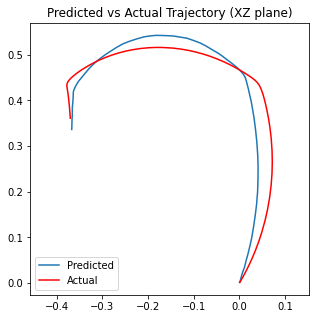
\includegraphics[height=1.8in]{images/result-examples/pose/trajectories/multiwarp/mw-epi-44.png}
    }
    \subfloat[Focal Stacks]{
        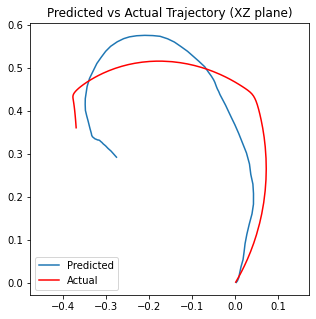
\includegraphics[height=1.8in]{images/result-examples/pose/trajectories/multiwarp/mw-fs-175-44.png}
    }
    \subfloat[Volumetric Images]{
        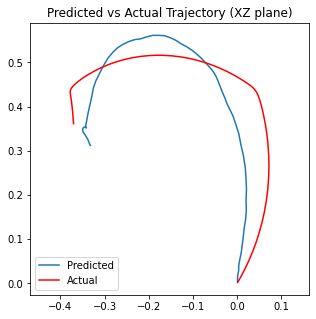
\includegraphics[height=1.8in]{images/result-examples/pose/trajectories/multiwarp/mw-stack-44.png}
    }
    \subfloat[Monocular]{
        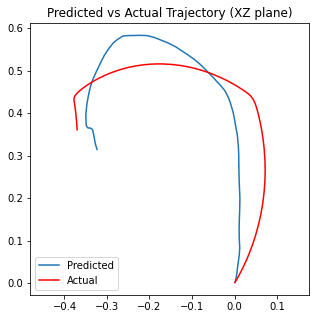
\includegraphics[height=1.8in]{images/result-examples/pose/trajectories/monocular/monocular-44.png}
    }
    \caption[Estimated and true trajectories for input sequence 44 using light field reconstruction]{Estimated and true trajectories for input sequence 44. Once again, tiled EPIs exhibit the most visually accurate trajectory, even picking up on the subtle corners that were missed by each of our other input methods.}
    \setcounter{subfigure}{0}
\end{figure}

\begin{table}[htbp]
    \caption{Mean Absolute Instantaneous Error and Cumulative Error}
    \centering
    \begin{tabular}{@{}lcc@{}}
        \toprule
        Input Method        & Absolute Instantaneous Error (mm)  & Cumulative Error (mm)  \\
        \midrule 
        Tiled EPIs & \textbf{7.61} & \textbf{50.61} \\
        Focal Stacks & 9.71 & 73.40 \\
        Volumetric Stacks & 10.50 & 110.04 \\
        Monocular & 12.90 & 122.23 \\
        \bottomrule
        
    \end{tabular}
\end{table}


% \subsection{Monocular Approach}

% Importantly, we have compared our results to the monocular approach using the algorithm suggested by \cite{zhou2017unsupervised}. In this instance, the pair of convolutional networks are not exposed to any sort of light field imagery - the input image is a single 2D image and the photometric warp is similarly performed on a single 2D image. 

% \begin{figure}[H]
%     \centering
%     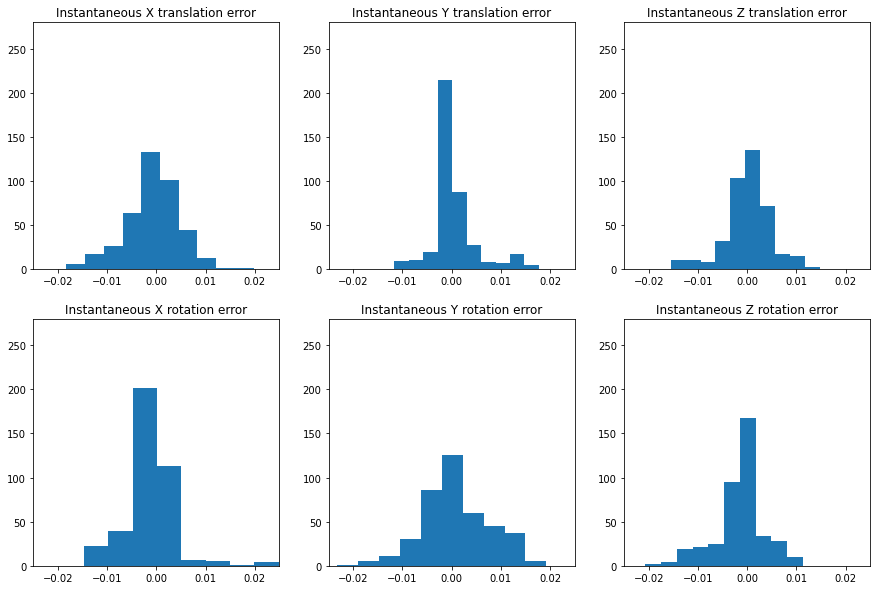
\includegraphics[width=\textwidth]{images/result-examples/pose/errors/singlewarp-stack.png}
%     \caption[Instantaneous errors for monocular imagery]{Instantaneous absolute errors when using \textbf{monocular imagery}.}
% \end{figure}

% \begin{figure}[H]
%     \centering
%     \subfloat[Sequence 16]{
%         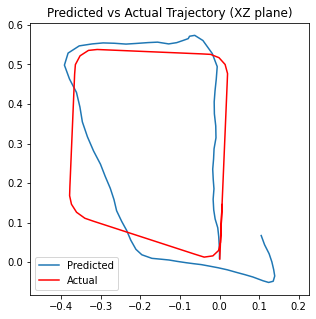
\includegraphics[height=2.7in]{images/result-examples/pose/trajectories/monocular/monocular-16.png}
%     }
%     \subfloat[Sequence 44]{
%         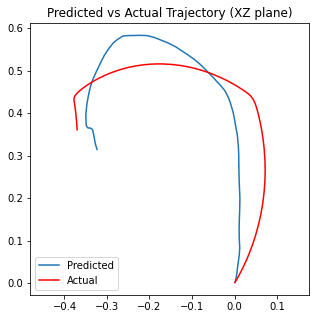
\includegraphics[height=2.7in]{images/result-examples/pose/trajectories/monocular/monocular-44.png}
%     }
%     \caption[Estimated and true trajectories for input sequences 16 and 44, using monocular imagery]{Estimated and true trajectories using monocular imagery.}
%     \setcounter{subfigure}{0}
% \end{figure}



\subsection{Comparison Between Approaches and Summary}

For ease of comparison, here we present graphical results for our three input formats, and two reconstruction approaches. Figures 5.7 and 5.8 show instantaneous and cumulative translational errors respectively, while Figure 5.9 shows instantaneous rotational errors. In all cases, tiled EPIs produce the smallest errors. 

\begin{figure}[H]
    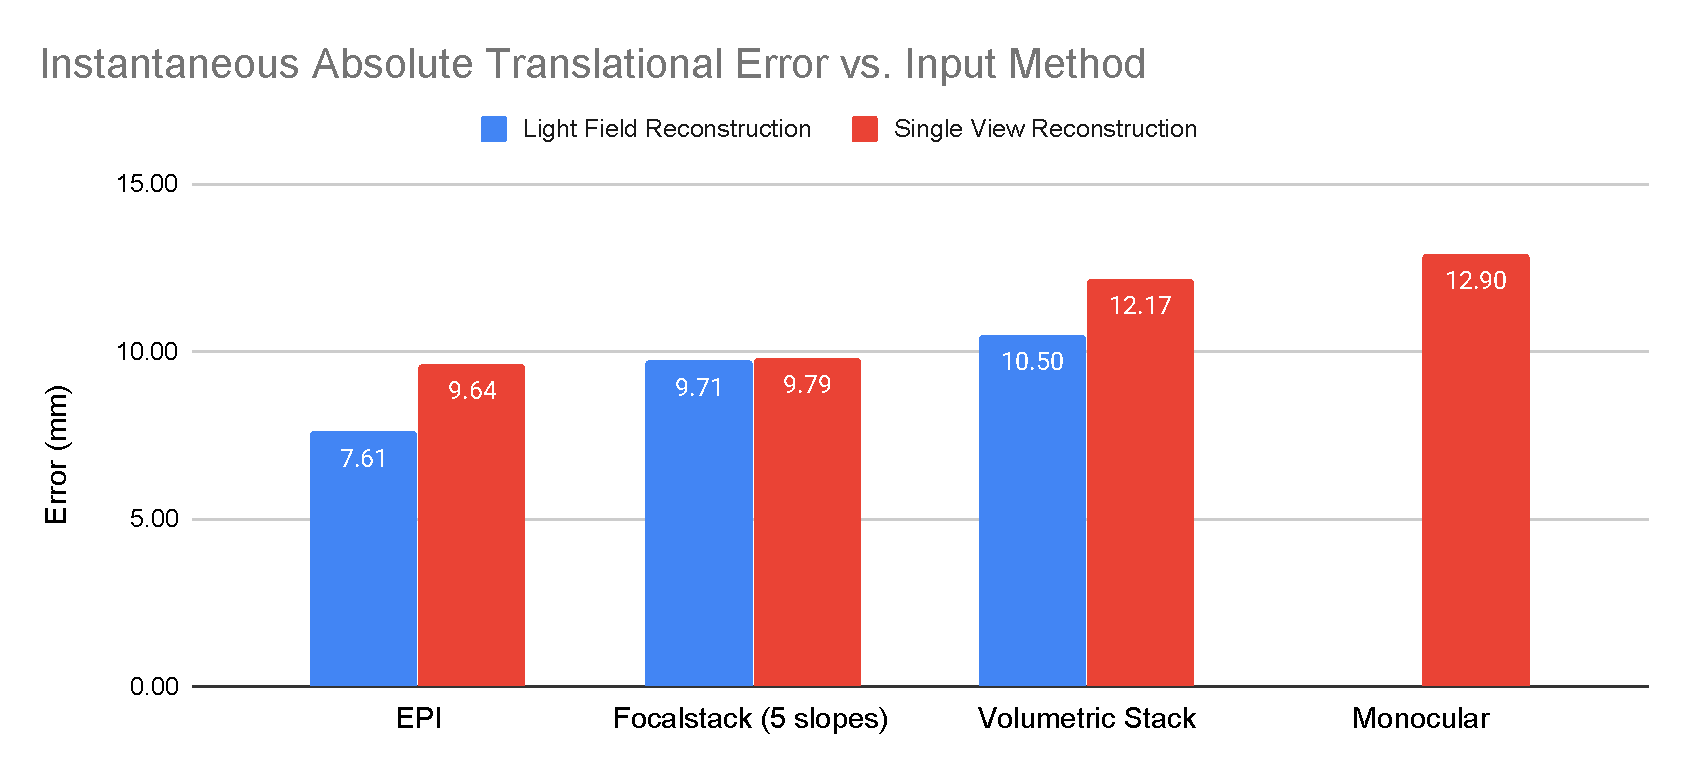
\includegraphics[width=\textwidth]{images/result-examples/bargraphs/iate-vs-inputmethod2.pdf}
    \caption[Instantaneous translational errors vs. input methods.]{We find that in terms of translational error, the light field reconstruction pipeline has an edge over the single-view warp variant in all three cases. Additionally, using tiled EPI's demonstrates the smallest translational error of the three input methods.}
\end{figure}
\begin{figure}[H]
    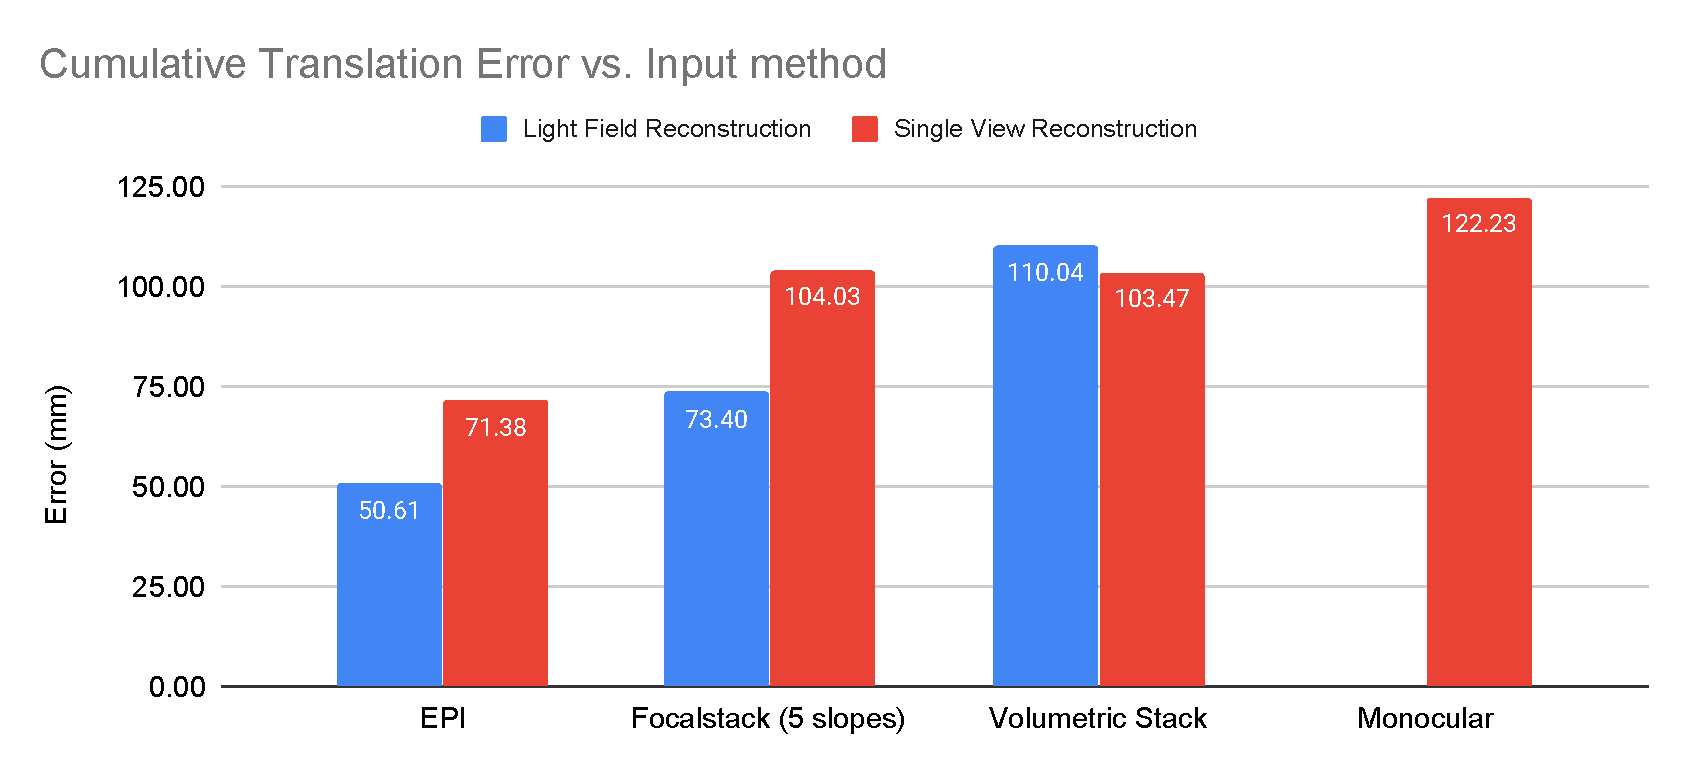
\includegraphics[width=\textwidth]{images/result-examples/bargraphs/cte-vs-input-method2.pdf}
    \caption[Cumulative translational errors vs. input methods.]{Similarly, we find that over the course of an entire video-sequence, tiled EPIs once again outperform all other input strategies. Over an entire video-sequence, the light field reconstruction pipeline generally outperforms the single-warp pipeline.}
\end{figure}
\begin{figure}[H]
    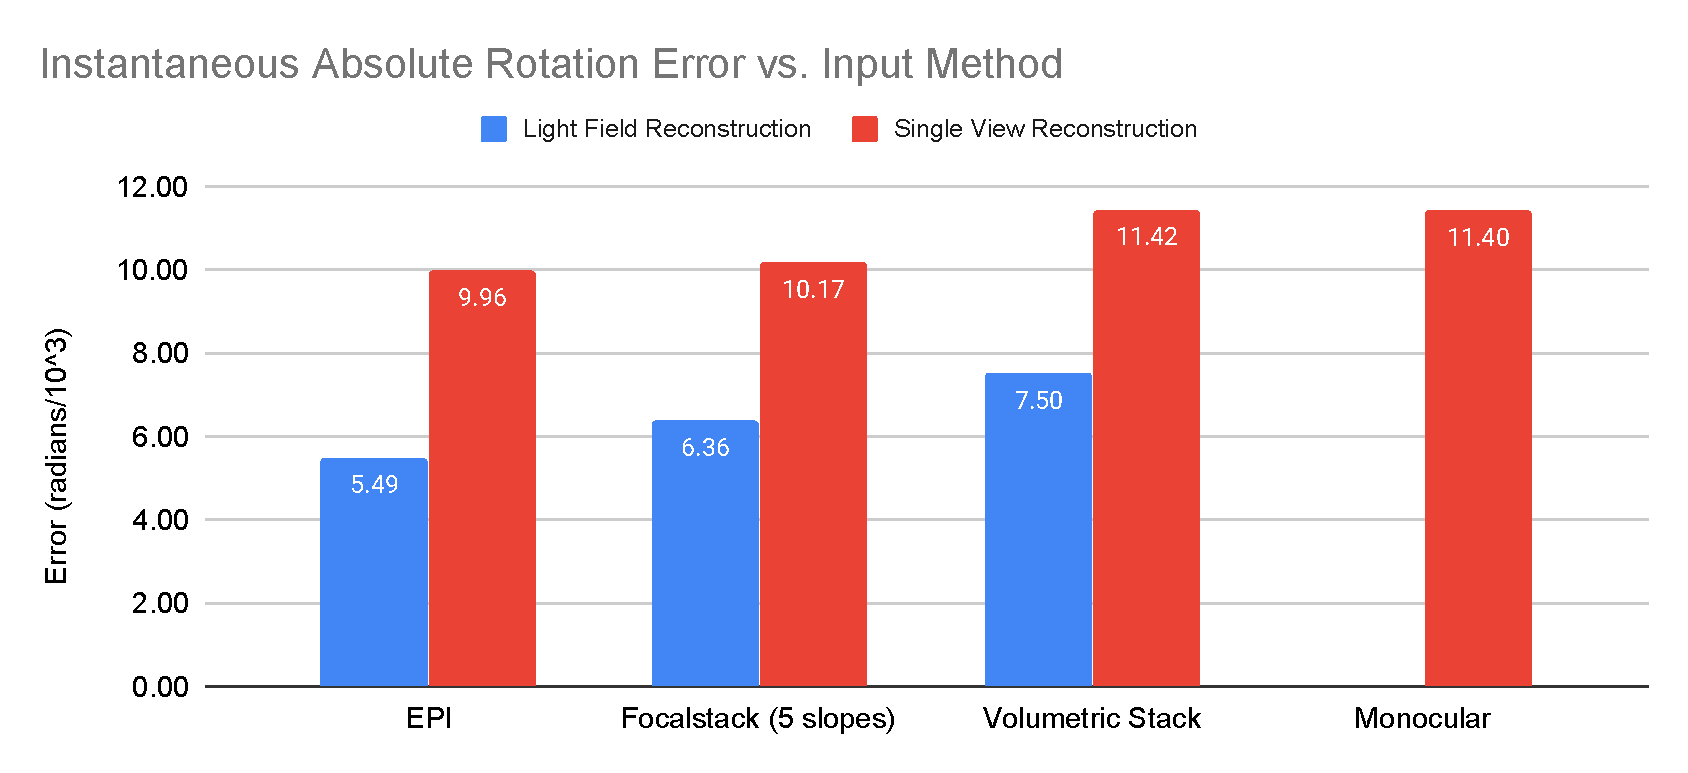
\includegraphics[width=\textwidth]{images/result-examples/bargraphs/iare-vs-input-method2.pdf}
    \caption[Instantaneous rotational error vs. input methods.]{We find that in rotational terms, light-field-reconstruction significantly outperforms the single-view-reconstruction pipeline. Similarly, we find that once again, the tiled EPI insertion strategy exhibits the smallest error in terms of rotation on our validation dataset.}
\end{figure}
\section{Depth and Photometric Reconstruction}

Aside from pose predictions and trajectories, our pipeline also generates depth-map predictions. In this section, we evaluate these outputs. Because our data acquisition methodology did not include the collection of ground-truth depth data, we must find more creative ways of evaluating depth. One way we can do this is by inspecting the visual quality of the depth maps, observing the artifacts and details resolved. For example, in the depth maps shown, we include a particularly challenging scenario that includes a wire-frame model of a flamingo. 

\begin{figure}[H]
    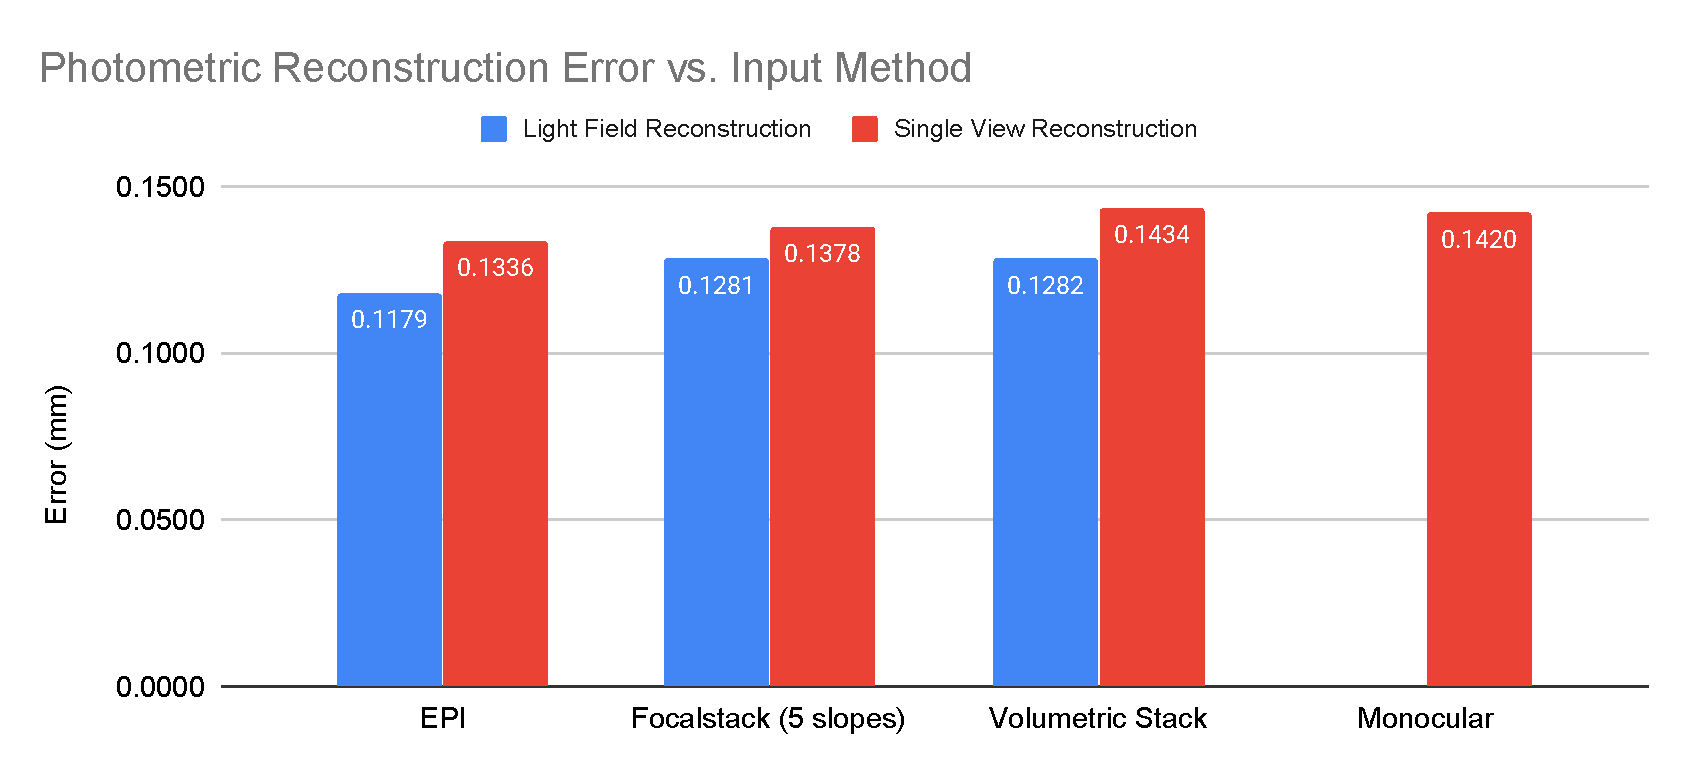
\includegraphics[width=\textwidth]{images/result-examples/bargraphs/photometric-error-vs-inputmethod2.pdf}
    \caption[Photometric reconstruction error vs. input methods]{The use of light-field-reconstruction to supervise the learning process consistently outperforms single-view reconstruction in terms of photometric error, for all of our tested input methods.}
\end{figure}

Another way we can evaluate the quality of our depth maps is to compare the photometric loss from image synthesis. Comparing the synthesised image with the ground-truth image, we can compute a difference-image which shows the magnitude of the error in rendering the synthesised image. Photometric error is measured as the difference between the ground truth pixel intensity, and the pixel intensity in the synthesised image, meaning that we can also summarise photometric loss as a single number, which is shown in Figure 5.10 - comparing different input methods.

\newgeometry{left=3cm,bottom=0.1cm}
\subsection{Single-View Reconstruction Approach}
Figure 5.11 shows depth map predictions for our three input methods, over a series of example frames from our testing dataset. Of the three input methods, using tiled EPIs exhibits the smoothest, most visually accurate frames, even picking up on holes in objects, and parts of a wire-frame flamingo.
\begin{figure}[H]
    \centering
    \subfloat[Input Image]{
        
\includegraphics[height=0in, width=1.4in]{images/blank.png}
    }
    \subfloat[Volumetric Stack]{
        
\includegraphics[height=0in, width=1.4in]{images/blank.png}
    }
    \subfloat[Focal Stack]{
        
\includegraphics[height=0in, width=1.4in]{images/blank.png}
    }
    \subfloat[Tiled EPIs]{
        
\includegraphics[height=0in, width=1.4in]{images/blank.png}
    }\\ 
    \subfloat{
        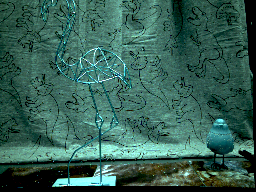
\includegraphics[height=1in]{images/result-examples/depth/16-18.png}
    }
    \subfloat{
        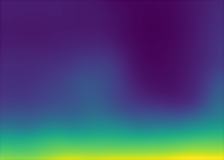
\includegraphics[height=1in]{images/result-examples/depth/singlewarp/stack/16-18.png}
    }
    \subfloat{
        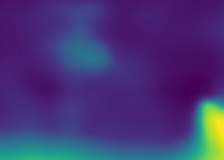
\includegraphics[height=1in]{images/result-examples/depth/singlewarp/focalstack-17-5/16-18.png}
    }
    \subfloat{
        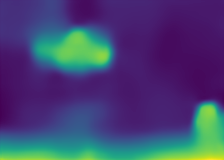
\includegraphics[height=1in]{images/result-examples/depth/singlewarp/epi/16-18.png}
    }\\ 
    \subfloat{
        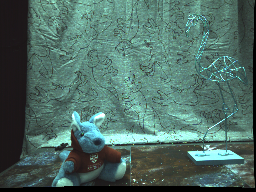
\includegraphics[height=1in]{images/result-examples/depth/16-50.png}
    }
    \subfloat{
        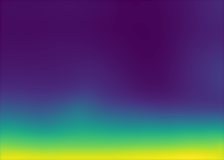
\includegraphics[height=1in]{images/result-examples/depth/singlewarp/stack/16-50.png}
    }
    \subfloat{
        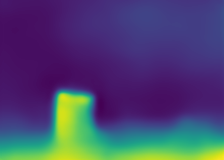
\includegraphics[height=1in]{images/result-examples/depth/singlewarp/focalstack-17-5/16-50.png}
    }
    \subfloat{
        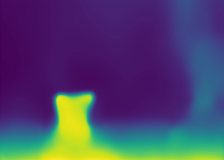
\includegraphics[height=1in]{images/result-examples/depth/singlewarp/epi/16-50.png}
    }\\
    \subfloat{
        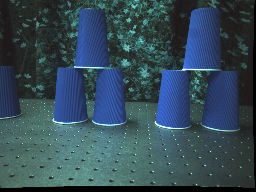
\includegraphics[height=1in]{images/result-examples/depth/44-0.png}
    }
    \subfloat{
        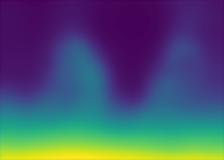
\includegraphics[height=1in]{images/result-examples/depth/singlewarp/stack/44-0.png}
    }
    \subfloat{
        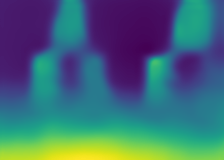
\includegraphics[height=1in]{images/result-examples/depth/singlewarp/focalstack-17-5/44-0.png}
    }
    \subfloat{
        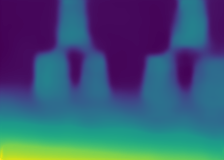
\includegraphics[height=1in]{images/result-examples/depth/singlewarp/epi/44-0.png}
    }\\
    \subfloat{
        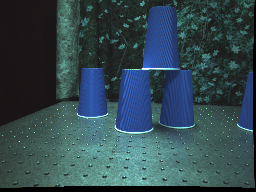
\includegraphics[height=1in]{images/result-examples/depth/44-40.png}
    }
    \subfloat{
        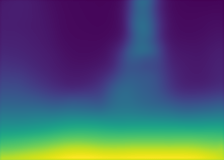
\includegraphics[height=1in]{images/result-examples/depth/singlewarp/stack/44-40.png}
    }
    \subfloat{
        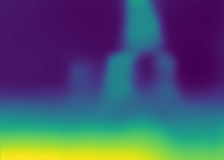
\includegraphics[height=1in]{images/result-examples/depth/singlewarp/focalstack-17-5/44-40.png}
    }
    \subfloat{
        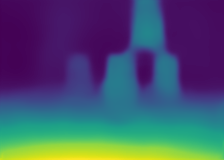
\includegraphics[height=1in]{images/result-examples/depth/singlewarp/epi/44-40.png}
    }\\
    \subfloat{
        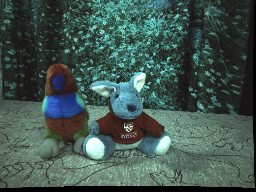
\includegraphics[height=1in]{images/result-examples/depth/50-10.png}
    }
    \subfloat{
        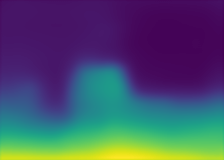
\includegraphics[height=1in]{images/result-examples/depth/singlewarp/stack/50-10.png}
    }
    \subfloat{
        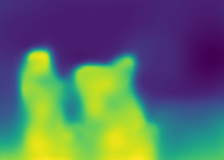
\includegraphics[height=1in]{images/result-examples/depth/singlewarp/focalstack-17-5/50-10.png}
    }
    \subfloat{
        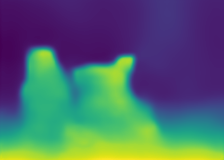
\includegraphics[height=1in]{images/result-examples/depth/singlewarp/epi/50-10.png}
    }\\
    \subfloat{
        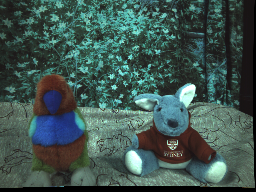
\includegraphics[height=1in]{images/result-examples/depth/51-69.png}
    }
    \subfloat{
        \includegraphics[height=1in]{images/result-examples/depth/singlewarp/stack/51-69.png}
    }
    \subfloat{
        \includegraphics[height=1in]{images/result-examples/depth/singlewarp/focalstack-17-5/51-69.png}
    }
    \subfloat{
        \includegraphics[height=1in]{images/result-examples/depth/singlewarp/epi/51-69.png}
    }
    \setcounter{subfigure}{0}
    \caption[Depth maps produced using single-view reconstruction]{Comparing depth maps estimated using each of our three input methods using single-view reconstruction, the tiled EPI input format appears to give the most visually accurate predictions, with edges resolved clearly, even capturing the appearance of the wireframe flamingo (first row) and some of the holes in between objects.}
    
\end{figure}
\restoregeometry

\newgeometry{left=3cm,bottom=0.1cm}
\subsection{Light Field Reconstruction Approach}

Similarly, we now show depth predictions when light field reconstruction is used for training the networks. Notably, only the output layer of the disparity network has changed - in other words, the only major difference is the formation of a supervising loss function. We see from Figure 5.12 that the depth maps are qualitatively more convincing with details resolved far more clearly.

\begin{figure}[H]
    \centering
    \subfloat[Input Image]{
        \includegraphics[height=0in, width=1.40in]{images/blank.png}
    }
    \subfloat[Volumetric Stack]{
        \includegraphics[height=0in, width=1.40in]{images/blank.png}
    }
    \subfloat[Focal Stack]{
        \includegraphics[height=0in, width=1.40in]{images/blank.png}
    }
    \subfloat[Tiled EPIs]{
        \includegraphics[height=0in, width=1.40in]{images/blank.png}
    }\\ 
    \subfloat{
        \includegraphics[height=1in]{images/result-examples/depth/16-18.png}
    }
    \subfloat{
        \includegraphics[height=1in]{images/result-examples/depth/multiwarp/stack/16-18.png}
    }
    \subfloat{
        \includegraphics[height=1in]{images/result-examples/depth/multiwarp/focalstack-17-5/16-18.png}
    }
    \subfloat{
        \includegraphics[height=1in]{images/result-examples/depth/multiwarp/epi/16-18.png}
    }\\ 
    \subfloat{
        \includegraphics[height=1in]{images/result-examples/depth/16-50.png}
    }
    \subfloat{
        \includegraphics[height=1in]{images/result-examples/depth/multiwarp/stack/16-50.png}
    }
    \subfloat{
        \includegraphics[height=1in]{images/result-examples/depth/multiwarp/focalstack-17-5/16-50.png}
    }
    \subfloat{
        \includegraphics[height=1in]{images/result-examples/depth/multiwarp/epi/16-50.png}
    }\\
    \subfloat{
        \includegraphics[height=1in]{images/result-examples/depth/44-0.png}
    }
    \subfloat{
        \includegraphics[height=1in]{images/result-examples/depth/multiwarp/stack/44-0.png}
    }
    \subfloat{
        \includegraphics[height=1in]{images/result-examples/depth/multiwarp/focalstack-17-5/44-0.png}
    }
    \subfloat{
        \includegraphics[height=1in]{images/result-examples/depth/multiwarp/epi/44-0.png}
    }\\
    \subfloat{
        \includegraphics[height=1in]{images/result-examples/depth/44-40.png}
    }
    \subfloat{
        \includegraphics[height=1in]{images/result-examples/depth/multiwarp/stack/44-40.png}
    }
    \subfloat{
        \includegraphics[height=1in]{images/result-examples/depth/multiwarp/focalstack-17-5/44-40.png}
    }
    \subfloat{
        \includegraphics[height=1in]{images/result-examples/depth/multiwarp/epi/44-40.png}
    }\\
    \subfloat{
        \includegraphics[height=1in]{images/result-examples/depth/50-10.png}
    }
    \subfloat{
        \includegraphics[height=1in]{images/result-examples/depth/multiwarp/stack/50-10.png}
    }
    \subfloat{
        \includegraphics[height=1in]{images/result-examples/depth/multiwarp/focalstack-17-5/50-10.png}
    }
    \subfloat{
        \includegraphics[height=1in]{images/result-examples/depth/multiwarp/epi/50-10.png}
    }\\
    \subfloat{
        \includegraphics[height=1in]{images/result-examples/depth/51-69.png}
    }
    \subfloat{
        \includegraphics[height=1in]{images/result-examples/depth/multiwarp/stack/51-69.png}
    }
    \subfloat{
        \includegraphics[height=1in]{images/result-examples/depth/multiwarp/focalstack-17-5/51-69.png}
    }
    \subfloat{
        \includegraphics[height=1in]{images/result-examples/depth/multiwarp/epi/51-69.png}
    }
    \setcounter{subfigure}{0}
    \caption[Depth maps produced using light field reconstruction]{Compared to the single-view reconstruction pipeline, these depth maps using the light field reconstruction pipeline resolve edges and details far more clearly. The tiled EPI input format once again captures the details of the wireframe flamingo most convincingly.}
\end{figure}
\restoregeometry


\subsection{Monocular Approach}
 We observe from Figure 5.13 that depth estimates using monocular imagery show far less detail and that the depth maps appear much smoother. This is to be expected, as no 3D information is preserved in a 2D image, meaning that only learned 2D features can be used to infer depth. 

\begin{figure}[H]
    \centering
    \subfloat[Input Image]{
        \includegraphics[height=0in, width=1.40in]{images/blank.png}
    }
    \subfloat[Depth Esimtate]{
        \includegraphics[height=0in, width=1.40in]{images/blank.png}
    }
    \subfloat[Input Image]{
        \includegraphics[height=0in, width=1.40in]{images/blank.png}
    }
    \subfloat[Depth Estimate]{
        \includegraphics[height=0in, width=1.40in]{images/blank.png}
    }\\ 
    \subfloat{
        \includegraphics[height=1in]{images/result-examples/depth/16-18.png}
    }
    \subfloat{
        \includegraphics[height=1in]{images/result-examples/depth/singlewarp/stack/16-18.png}
    }
    \subfloat{
        \includegraphics[height=1in]{images/result-examples/depth/16-50.png}
    }
    \subfloat{
        \includegraphics[height=1in]{images/result-examples/depth/singlewarp/stack/16-50.png}
    }\\
    \subfloat{
        \includegraphics[height=1in]{images/result-examples/depth/44-0.png}
    }
    \subfloat{
        \includegraphics[height=1in]{images/result-examples/depth/singlewarp/stack/44-0.png}
    }
    \subfloat{
        \includegraphics[height=1in]{images/result-examples/depth/44-40.png}
    }
    \subfloat{
        \includegraphics[height=1in]{images/result-examples/depth/singlewarp/stack/44-40.png}
    }\\
    \subfloat{
        \includegraphics[height=1in]{images/result-examples/depth/50-10.png}
    }
    \subfloat{
        \includegraphics[height=1in]{images/result-examples/depth/singlewarp/stack/50-10.png}
    }
    \subfloat{
        \includegraphics[height=1in]{images/result-examples/depth/51-69.png}
    }
    \subfloat{
        \includegraphics[height=1in]{images/result-examples/depth/singlewarp/stack/51-69.png}
    }
    \setcounter{subfigure}{0}
    \caption[Depth maps using monocular imagery.]{Unsurprisingly, monocular imagery produces the least visually convincing depth maps. Simple features like the flatness of the table and blobs of objects in front of the camera appear, but edges and discontinuities are not captured well.}
\end{figure}


\subsection{Qualitative Analysis}

Another useful result for inspection is the \textit{difference image} - this shows the pixel-wise difference between the photometrically warped output of our algorithm, and the target image. Inspecting the two images side-by-side and discerning the difference is a challenging task, and so with the aid of the difference image we make the difference between the two images clearer.

Below, we show some examples of the target image (the image to be reconstructed), the output from photometric reconstruction, and the difference image. We show examples for the best-performing version of our algorithm - using epipolar plane images as the input format with light-field-reconstruction used as the training pipeline. 

\begin{figure}[H]
    \centering
    \subfloat[Target Image]{
        \includegraphics[height=0in, width=1.85in]{images/blank.png}
    }
    \subfloat[Reconstructed Image]{
        \includegraphics[height=0in, width=1.85in]{images/blank.png}
    }
    \subfloat[Difference]{
        \includegraphics[height=0in, width=1.85in]{images/blank.png}
    }\\
    \subfloat{
        \includegraphics[height=1.4in]{images/result-examples/warps/seq16/input.png}
    }
    \subfloat{
        \includegraphics[height=1.4in]{images/result-examples/warps/seq16/warped.png}
    }
    \subfloat{
        \includegraphics[height=1.4in]{images/result-examples/warps/seq16/diff.png}
    }\\
    \subfloat{
        \includegraphics[height=1.4in]{images/result-examples/warps/seq44/input.png}
    }
    \subfloat{
        \includegraphics[height=1.4in]{images/result-examples/warps/seq44/warped.png}
    }
    \subfloat{
        \includegraphics[height=1.4in]{images/result-examples/warps/seq44/diff.png}
    }\\ 
    \subfloat{
        \includegraphics[height=1.4in]{images/result-examples/warps/seq51/input.png}
    }
    \subfloat{
        \includegraphics[height=1.4in]{images/result-examples/warps/seq51/warped.png}
    }
    \subfloat{
        \includegraphics[height=1.4in]{images/result-examples/warps/seq51/diff.png}
    }\\
    \caption[Inspecting the difference image from photometric synthesis]{Difference images reveal where the largest errors occurred in photometric synthesis. The most apparent errors occur around 3D discontinuities and high-texture parts of the image.}
\end{figure}

Notably, we observe that the reconstructed image exhibits reduced clarity compared to the target image. Not unexpectedly, we find that the largest errors occur around 3D depth discontinuities - where occluders coming into and out-of view affect the correctness of our image-based sampling strategy. Similarly, textured regions of the image also exhibit heavy losses, as even small errors in the pose and depth estimate exacerbate the photometric warp error around these regions.

\section{Summary of Results}

Table 5.3 is a summary of results from this chapter, including odometry and photometric errors. Algorithmic bandwidth is an important consideration in real-time systems such as robotics, and so we also report the time required for both inference and training. We report the execution time for Python code running on an Intel i5 4460 CPU at 3.2 GHz, with tensor computations taking place on a GeForce GTX 1050Ti GPU. Inference is near-realtime for full framerate video, supporting up to 5 frames per second, which is competitive with the existing monocular approach (which we measure at just under 10 frames per second). The following acronyms are used in the table headings.

\begin{itemize}
    \item {AITE: Absolute instantaneous translational error}
    \item {AIRE: Absolute instantaneous rotational error}
    \item {CE: Cumulative translational error}
    \item {PWE: Photometric warp error}
\end{itemize}


\begin{table}[htbp]
    \caption{Summary of Odometry and Photometric Warp Errors, and Execution Times}
    \centering
    \hspace*{-0.4cm}
    \begin{tabular}{@{}lcccccc@{}}
        \toprule
        Input Method       & AITE (mm) & AIRE (mm) & CE (mm)   & PWE  & Infer (ms) & Train (hrs) \\
        \midrule 
        \multicolumn{3}{l}{\textit{Single View Reconstruction Pipeline}}\\
        Tiled EPIs & 9.64 & 9.96 & 71.38 & 0.1336 & 154 & 17.9 \\
        Focal Stacks & 9.79 & 10.17 & 104.03  & 0.1378 & 205 & 25.0 \\
        Volumetric Stacks & 12.17 & 11.42 & 103.47 & 0.1434 & 112 & 17.6\\
        \midrule 
        \multicolumn{3}{l}{\textit{Light Field Reconstruction Pipeline}}\\
        Tiled EPIs & \textbf{7.61} & \textbf{5.49} & \textbf{50.61} & \textbf{0.1179} & 199 & 29.5 \\
        Focal Stacks & 9.71 & 6.36 & 73.40 & 0.1281 & 264 & 30.4 \\
        Volumetric Stacks & 10.50 & 7.50 & 110.04 & 0.1282 & 121 & 25.4 \\
        \midrule 
        \multicolumn{3}{l}{\textit{Monocular Approach}}\\
        Monocular Image & 12.90 & 11.40 & 122.23 & 0.1420 & \textbf{110} & \textbf{17.6} \\
        \bottomrule
        
    \end{tabular}
\end{table}




























